%-------------------------------------------------------------------------------
\chapter[How to]{How to?}
%-------------------------------------------------------------------------------
\pagebreak
%-------------------------------------------------------------------------------
\section{Compute sediment fluxes through a given section(s)}
%-------------------------------------------------------------------------------
Use the keywords {\ttfamily FLUXLINE} (logical type, set to {\ttfamily NON} by default) and {\ttfamily FLUXLINE INPUT FILE} (character type).

The format of the {\ttfamily FLUXLINE INPUT FILE} includes (see Figure~\ref{fig:fluxline_example}):
\begin{itemize}
\item The number of fluxlines (integer)
\item The definition of the fluxlines, given by:
  \begin{itemize}
  \item The specification of two points of the fluxline (\texttt{fluxline\_x1, fluxline\_y1, fluxline\_x2, fluxline\_y2}), followed by
  \item the definition of the bounding box (\texttt{box\_x1, box\_y1, box\_x2, box\_y2})
  \item An integer (value not used)
  \end{itemize}
\end{itemize}

An example of the {\ttfamily FLUXLINE INPUT FILE} is given below:

\begin{lstlisting}[frame=trBL]
5
94.0   31.2  99.0  31.2 95.0  31.0  98.0  31.6 1
94.0   42.5  99.0  42.5 96.0  42.0  98.0  43.0 1
101.0  42.5  107.0 42.5 104.0 42.0  106.0 43.0 1
101.0  31.2  107.0 31.2 104.0 31.0  106.0 31.6 1
100.0  45.0  102.0 48.0 100.0 46.0  102.0 47.5 1  
\end{lstlisting}     

\begin{figure}[H]
\begin{center}
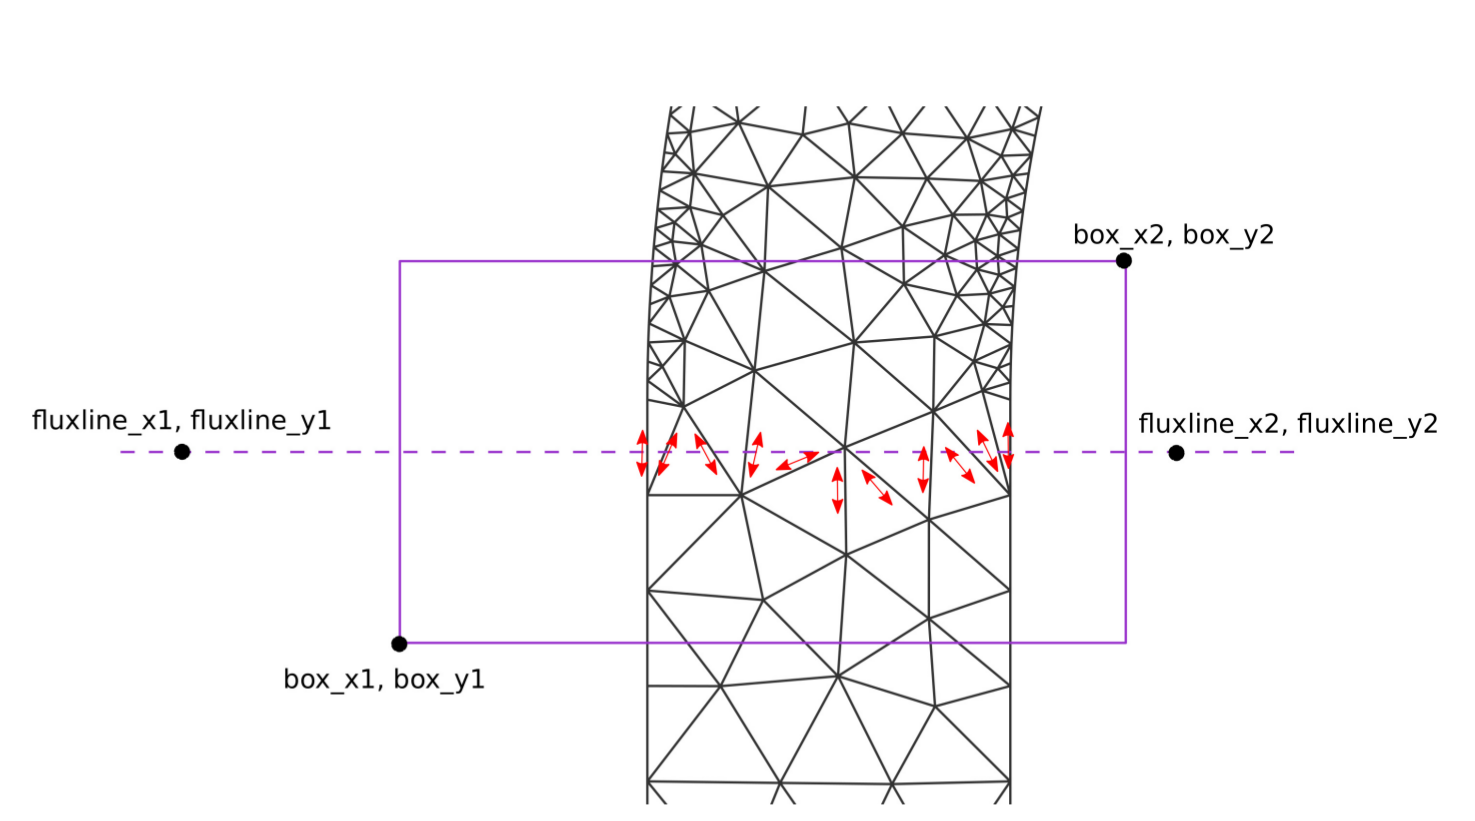
\includegraphics[scale=0.25,angle=0]{graphics/fluxline_example.png}
\caption{Description of a single fluxline and edge fluxes (red).}\label{fig:fluxline_example}
\end{center}
\end{figure}

Further details can be found in Stadler L. (2015) \textit{Calculating correct water and sediment fluxes in TELEMAC2D and SISYPHE}. Proceedings of the 22$^{th}$
Telemac \& Mascaret User Club, STFC Daresbury Laboratory, UK, 13-16 October.

%\pagebreak
%-------------------------------------------------------------------------------
\section{Implement a new bedload transport formula}
%-------------------------------------------------------------------------------
To implement a new bedload transport formula, the keyword {\ttfamily BED-LOAD TRANSPORT FORMULA} must be set to {\ttfamily = 0}. The Fortran subroutine must be added into the fortran file of \textsc{Telemac-2d} or \textsc{Telemac-3d}, keyword {\ttfamily FORTRAN FILE}.

The template subroutine is called \texttt{qsfrom.f} and can be found in the folder \texttt{/sources/sisyphe}
\begin{lstlisting}[frame=trBL]
!                    ***************** 
                     SUBROUTINE QSFORM 
!                    ***************** 
     &(U2D, V2D, TOB, HN, XMVE, TETAP, MU, NPOIN, DM,  
     & DENS, GRAV, DSTAR, AC, QSC, QSS) 
! 
!***********************************************************************
! SISYPHE   V6P2                                   21/07/2011 
!***********************************************************************
! 
!brief    ALLOWS THE USER TO CODE THEIR OWN BEDLOAD TRANSPORT 
!+                FORMULATION, BEST SUITED TO THEIR APPLICATION. 
! 
!~~~~~~~~~~~~~~~~~~~~~~~~~~~~~~~~~~~~~~~~~~~~~~~~~~~~~~~~~~~~~~~~~~~~~~~
!~~~~~~~~~~~~~~~~~~~~~~~~~~~~~~~~~~~~~~~~~~~~~~~~~~~~~~~~~~~~~~~~~~~~~~~
! 
      USE INTERFACE_SISYPHE, EX_QSFORM => QSFORM 
!     USE DECLARATIONS_SISYPHE 
      USE BIEF 
      IMPLICIT NONE 
      INTEGER LNG,LU 
      COMMON/INFO/LNG,LU 
! 
!+-+-+-+-+-+-+-+-+-+-+-+-+-+-+-+-+-+-+-+-+-+-+-+-+-+-+-+-+-+-+-+-+-+-+-+
! 
      TYPE(BIEF_OBJ),   INTENT(IN)    :: U2D,V2D,TOB,HN,TETAP,MU 
      TYPE(BIEF_OBJ),   INTENT(INOUT) :: QSC, QSS 
      INTEGER,          INTENT(IN)    :: NPOIN 
      DOUBLE PRECISION, INTENT(IN)    :: XMVE, DM, DENS, GRAV, DSTAR, AC
! 
!+-+-+-+-+-+-+-+-+-+-+-+-+-+-+-+-+-+-+-+-+-+-+-+-+-+-+-+-+-+-+-+-+-+-+-+
! 
! 
      INTEGER          :: I 
      DOUBLE PRECISION :: C1, C2, T 
      DOUBLE PRECISION, PARAMETER :: ACOEFF = 0.004D0!Sediment transport param (m^2s^-1)
! 
!======================================================================!
!======================================================================!
!                               PROGRAM                                !
!======================================================================!
!======================================================================!
! 
!     GRASS (1981) TYPE 
!      
      DO I = 1, NPOIN 
 
        QSC%R(I) = ACOEFF * U2D%R(I) * (U2D%R(I)**2+V2D%R(I)**2) ! 1D Grass (1981)  
        QSS%R(I) = 0.D0                                          ! Zero suspended load
 
      END DO 
! 
! 
!-----------------------------------------------------------------------
! 
      RETURN 
      END
\end{lstlisting}      

%\pagebreak
%-------------------------------------------------------------------------------
%\section{Define a rigid bed}
%-------------------------------------------------------------------------------
%TODO
%\subsection{Data from selafin file}
%\subsection{Data coded by the user in the fortran file}

%\pagebreak
%-------------------------------------------------------------------------------
\section{Print a new output variable in the selafin file}
%-------------------------------------------------------------------------------
\begin{itemize}
\item Declare the {\ttfamily PRIVE} variable, for example as:
  
{\ttfamily USE DECLARATIONS\_SISYPHE, ONLY : PRIVE}

\item Use the following expression to include the variable you want to visualize:

{\ttfamily PRIVE\%ADR(N)\%P\%R(K) = [Here the variable you want to visualize]}, where {\ttfamily N} is the number of variables that you want to visualize and {\ttfamily K} is the number of nodes.  

\item In the \sisyphe's steering file you can use the flags {\ttfamily'A'} or {\ttfamily'G'} to visualize the {\ttfamily PRIVE} variable, for example as:
  
{\ttfamily VARIABLES FOR GRAPHIC PRINTOUTS='U,V,S,H,B,Q,M,E,QSBL,TOB,MU,A'}
\end{itemize}

The default name {\ttfamily PRIVE 1} (for {\ttfamily N=1}) can be modified in the subroutine {\ttfamily nomvar\_sisyphe.f}.

\begin{lstlisting}[frame=trBL]
DO K=1, NPOIN
  PRIVE%ADR(1)%P%R(K) = [variable to visualize]
ENDDO  
\end{lstlisting}  

%\pagebreak
%-------------------------------------------------------------------------------
\section{Introduce a new keyword}
%-------------------------------------------------------------------------------
\begin{itemize}
\item In {\ttfamily declarations\_sisyphe.f} declare the variable to be called from a keyword e.g. {\ttfamily HMIN\_BEDLOAD}
\item In {\ttfamily lecdon\_sisyphe.f} declare .... {\ttfamily HMIN\_BEDLOAD=MOTREA(ADRESS(2,52))}
\item Declaration in the modified subroutine through {\ttfamily USE DECLARATIONS\_SISYPHE, ONLY : HMIN\_BEDLOAD}
\end{itemize}


%\pagebreak
%-------------------------------------------------------------------------------
\section{Read and use a variable from a selafin file}
%-------------------------------------------------------------------------------
Case of spatially distributed sediment zones

\begin{itemize}
\item Create the different zones with, e.g. BlueKenue
\item Add in your steering file:
  \begin{lstlisting}[frame=trBL]
NUMBER OF PRIVATE ARRAYS = 1
NAMES OF PRIVATE VARIABLES= 'ZONE                            '
\end{lstlisting}
(32 characters)%\textvisiblespace\textvisiblespace\textvisiblespace
\item Modify the subroutine \texttt{init\_compo.f}, for example:
\begin{lstlisting}[frame=trBL]
      DO J=1,NPOIN
      NCOUCHES(J)=1
	  IF(PRIVE%ADR(1)%P%R(J).EQ.1.D0) THEN
	  AVAIL(J,1,1)=1.D0
	  AVAIL(J,1,2)=0.D0
	  ELSEIF(PRIVE%ADR(1)%P%R(J).EQ.2.D0) THEN
	  AVAIL(J,1,1)=0.D0
	  AVAIL(J,1,2)=1.D0	 
	  ELSE 
	  AVAIL(J,1,1)=0.5D0
	  AVAIL(J,1,2)=0.5D0
	  ENDIF
      ENDDO
\end{lstlisting}
\end{itemize}


%\pagebreak
%-------------------------------------------------------------------------------
%\section{Define the soil stratigraphy (init\_compo)}
%-------------------------------------------------------------------------------
%TODO

%\pagebreak
%-------------------------------------------------------------------------------
\section{Suppress bed updating}
%-------------------------------------------------------------------------------
Set \telkey{STATIONARY MODE = YES} (logical type, set to {\ttfamily = NO} by default)           


%\pagebreak
%-------------------------------------------------------------------------------
\section{Using a non-declared variable in a Sisyphe's subroutine}
%-------------------------------------------------------------------------------
If you want to use, for example, parameter \texttt{NPTFR} and the table \texttt{NBOR(NPTFR)} in the subroutine NOEROD,
declare:

\texttt{USE DECLARATIONS\_SISYPHE, ONLY : NPTFR, MESH}

\texttt{INTEGER, POINTER :: NBOR(:)}

Then the following alias can be declared:

\texttt{NBOR=>MESH\%NBOR\%I}

%\pagebreak
%-------------------------------------------------------------------------------
\section{Prevent erosion when water depth is smaller than a threshold value}
%-------------------------------------------------------------------------------
At for example intertidal wetlands with flooding and drying or tidal areas, the bottom friction could be very high when the water depth is very small, even for small velocities, leading to high and unphysical erosion rates. To prevent that, the keyword \telkey{MINIMAL VALUE OF THE WATER HEIGHT} can be used (the value by default is $1.0^{-3}$m). This keyword is activated when \telkey{TIDAL FLATS = YES}.
